\documentclass[a5paper]{article}
\usepackage[a5paper, top=8mm, bottom=8mm, left=8mm, right=8mm]{geometry}

\usepackage{polyglossia}
\setdefaultlanguage[babelshorthands=true]{russian}

\usepackage{fontspec}
\setmainfont{FreeSerif}
\newfontfamily{\russianfonttt}[Scale=0.7]{DejaVuSansMono}

\usepackage[font=scriptsize]{caption}

\usepackage{amsmath}
\usepackage{amssymb,amsfonts,textcomp}
\usepackage{color}
\usepackage{array}
\usepackage{hhline}
\usepackage{cite}
\usepackage{verse}

\usepackage[hang,multiple]{footmisc}
\renewcommand{\footnotelayout}{\raggedright}

\PassOptionsToPackage{hyphens}{url}\usepackage[xetex,linktocpage=true,plainpages=false,pdfpagelabels=false]{hyperref}
\hypersetup{colorlinks=true, linkcolor=blue, citecolor=blue, filecolor=blue, urlcolor=blue, pdftitle=1, pdfauthor=, pdfsubject=, pdfkeywords=}

\usepackage{tabu}

\usepackage{graphicx}
\usepackage{indentfirst}
\usepackage{multirow}
\usepackage{subfig}
\usepackage{footnote}
\usepackage{minted}

\sloppy
\pagestyle{plain}

\title{Domain-Driven Design, стратегические аспекты}
\author{Юрий Литвинов\\\small{yurii.litvinov@gmail.com}}

\date{}

\begin{document}

\maketitle
\thispagestyle{empty}

\section{Целостность модели}

Центральной идеей методологии предметно-ориентированного проектирования является единая модель предметной области и единый язык, что хорошо и правильно, но если над проектом работает сотня человек, это проблематично. Собрать всех на одной кухне, чтобы они могли оттачивать единый язык, физически невозможно, особенно если они на самом деле говорят на разных языках и сидят на разных континентах. В этой лекции речь пойдёт о том, как применять предметно-ориентированное проектирование к проектам, разрабатывающимся несколькими командами, о том, как вообще разрабатывать большие проекты, какие архитектурные проблемы при этом появляются и как их можно решать. Эта лекция по сути является кратким пересказом части IV книги <<Предметно-ориентированное проектирование (DDD). Структуризация сложных программных систем>>, Э. Эванс, и заканчивает рассказ о книге.

Итак, предметно-ориентированное проектирование в случае проекта, над которым работают несколько команд, сталкивается с проблемой того, что команды неизбежно имеют разные видения продукта. Эту проблему можно решать, 

\begin{itemize}
    \item либо поддерживая модель интегрированной --- но тогда затраты на поддержание её целостности будут слишком велики (в идеале --- все команды должны будут непосредственно общаться со всеми остальными, и каждое изменение в модели утверждаться остальными командами), при этом модель наверняка получится слишком общей, чтобы быть полезной;
    \item либо приняв ситуацию как должное и разрешив модели быть фрагментированной --- но тогда это неизбежно затруднит переиспользование кода в рамках проекта и интеграцию системы.
\end{itemize}

При этом бесконтрольное существование модели может привести к ошибкам, связанным с разным пониманием командами нюансов сущностей модели. Эрик Эванс приводил в книжке хороший пример, когда над системой работало несколько команд, и одной из них потребовалась абстракция для платежа клиента. Оказалось, что в коде уже был класс <<Платёж>>, разработанный другой командой, ну и, понятно, его решили переиспользовать. Парочки полей не хватало, одно называлось не совсем так, как надо, но ладно, в конце концов, какое имеет значение конкретное название. Однако система через пару дней начала внезапно падать, в модуле оплаты счетов субподрядчику, для которого изначально был разработан класс <<Платёж>>, в частности, на генерации налоговых отчётов. Стали разбираться, обнаружили в системе странные платежи, которые никто не вводил и которые не имели никакого смысла. Оказалось, что система крешилась из-за того, что у странных платежей не было заполнено поле <<необлагаемый процент>>, несмотря на то, что система требовала его заполнености и сама подставляла туда значение по умолчанию при создании платежа. Выяснилось, что это действительно были платежи клиентов, и для них действительно поле <<необлагаемый процент>> не имело смысла, поэтому просто не заполнялось. И эти платежи тоже попадали в вычисление налоговой отчётности (потому что они платежи же!) и всё падало.

Это выглядит как какая-то частная проблема, но корень зла тут вполне системный --- две команды использовали одну сущность в разных, хоть и похожих, смыслах. И не имели никакого механизма, позволявшего выявить заранее несоответствие значений, которые команды вкладывали в термин <<Платёж>>. Решением проблемы стало создание двух отдельных абстракций <<Платёж поставщику>> и <<Платёж клиента>> и договорённость более не мешать друг другу.

\subsection{Ограниченный контекст}

Командам из примера про <<Платёж>> могла бы помочь заранее достигнутая договорённость о границах их предметных областей и правилах переиспользования кода. В предметно-ориентированном проектировании для этого вводится понятие \textit{<<Ограниченный контекст>>}. Ограниченный контекст (Bounded context) --- это кусок предметной области (и, соответственно, реализующего её кода), в которой применима единая модель предметной области. Всё, что внутри ограниченного контекста, должно следовать этой единой модели, иметь единый язык и т.п., всё, что вне --- не должно делать никаких предположений о модели и не имеет право её без спроса переиспользовать. То есть, ограниченный контекст --- это что-то вроде атомарной области проекта, над которой работает одна команда (как клетка в живом организме, простите за банальную метафору). Разделение системы на ограниченные контексты обычно следует организационной структуре проекта, которая, в свою очередь, чаще всего следует высокоуровневой структуре системы. Например, в одном из проектов, в котором работал автор, по созданию средства автоматизированного реинжиниринга, была группа синтаксического анализа, группа извлечения бизнес-правил, группа генерации кода. Каждая группа имела собственный ограниченный контекст, свою терминологию и своё видение задачи, и интегрировалась с другими с помощью вполне определённых интерфейсов. Что происходило внутри, было делом каждой команды --- например, группа извлечения бизнес-правил занималась вообще какими-то магическими алгоритмами статического анализа программ, которые никто, кроме них, не понимал.

Внутри одного ограниченного контекста может работать довольно большое количество людей, между которыми также может возникнуть недопонимание, напряжение при попытке поддержания единого видения и т.п. Практика показывает, что 3-4 человека, тесно работая вместе, обычно могут договориться, но делить систему на ограниченные контексты по 3-4 человека оказывается непрактично. Поэтому в рамках ограниченного контекста практикуют \textit{<<непрерывную интеграцию>>} в её классическом понимании --- слияние изменений в основную ветку раз в несколько часов, постоянную (после каждого коммита) сборку и запуск юнит-тестов, обеспечение высокого тестового покрытия, непрерывное общение в рамках команды. Всё это позволяет быстро понять наличие проблем в понимании модели внутри ограниченного контекста и устранить их.

Для интеграции с другими ограниченными контекстами могут использоваться \textit{<<карты контекстов>>} (Context map). Карта контекстов фиксирует, как понятие из одной модели в рамках одного ограниченного контекста транслируется в понятие из другой модели из другого контекста. Карты трансляции обычно просто описываются на естественном языке (с применением терминов единых языков интегрируемых моделей), но могут и использоваться диаграммы такого примерно вида:

\begin{center}
    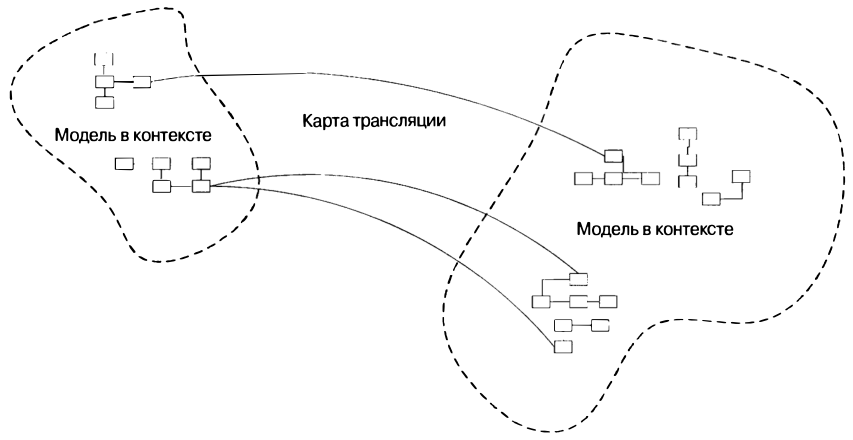
\includegraphics[width=0.7\textwidth]{contextMap.png}
\end{center}

Вот любимый Эриков Эвансом пример про сервис грузоперевозок, показывающий взаимосвязь ограниченных контекстов в рамках одной задачи: 

\begin{center}
    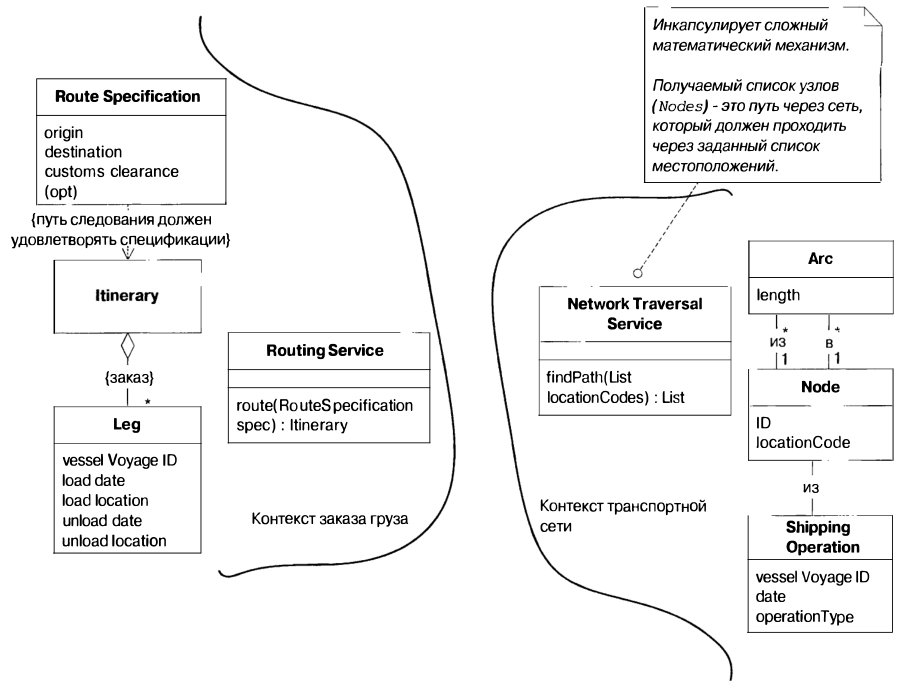
\includegraphics[width=0.8\textwidth]{contextBoundariesExample.png}
\end{center}

Есть команда, занимающаяся бизнес-логикой сервиса прокладки маршрута. Она оперирует понятиями <<Спецификация маршрута>>, <<Маршрут>>, <<Перевозка>> и использует <<Сервис прокладки маршрута>> для вызова кода второй команды, который собственно составляет маршрут перевозки между двумя точками. Вторая команда работает в терминах алгоритмов на графах, она ничего не знает и не хочет знать про перевозки, спецификации маршрута и конкретные корабли или поезда, везущие грузы. У них есть узлы и дуги с весами, узлы привязаны к координатам на местности и в узлах можно осуществлять погрузочно-разгрузочные операции над некоторыми абстрактными транспортными средствами, идентифицируемыми своим кодом. Это позволяет второй команде переиспользовать существующие библиотечные реализации графов и алгоритмов на них, не мучаясь со спецификой предметной области. Но это, естественно, требует определённых усилий на интеграцию, поскольку <<Сервис прокладки маршрута>> со стороны первой команды должен выполнять трансляцию в термины <<Сервиса поиска пути>> второй команды и обратно, и о том, как работают эти сервисы, команды должны чётко договориться. Зато всё, что находится за этими сервисами, может разрабатываться независимо. Что, конечно, приводит к дубликации кода, потому что Leg и Arc, по сути, выражают одно и то же понятие, но в данном случае это абсолютно осмысленно --- команды могут работать параллельно, не мешать друг другу и не мешать разные понятия в одну кучу.

\subsection{Паттерны интеграции контекстов}

Есть некоторые типичные ситуации, в которых возможны разные степени интеграции моделей предметной области и разные способы действий, необходимых, чтобы этой интеграции достичь и при этом не навредить разработке. Эванс в своей книге выделяет несколько подходов и даёт им имена (поэтому их можно рассматривать как что-то вроде паттернов интеграции контекстов). Выбор подхода, который стоит применять, зависит от конкретной ситуации и обстоятельств, скорее всего, не зависящих от команды. Поэтому стремиться к высокой интеграции контекстов не всегда стоит, и один из официальных подходов к интеграции --- это отказаться от интеграции вообще.

\subsubsection{Общее ядро}

Первый рассматриваемый здесь паттерн интеграции --- <<Общее ядро>> (Shared Kernel) --- предполагает наиболее тесную интеграцию, кроме объединения двух ограниченных контекстов в один. Такой подход предполагает выделение общей части двух ограниченных контекстов и совместную реализацию элементов модели оттуда:

\begin{center}
    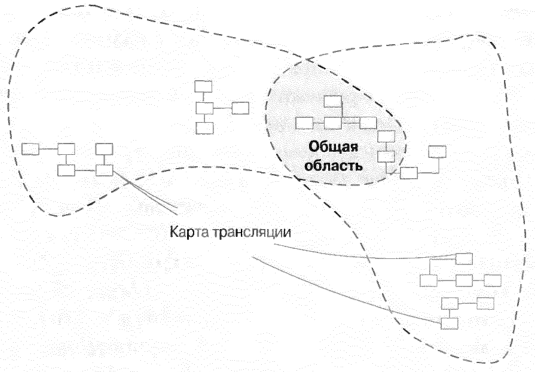
\includegraphics[width=0.7\textwidth]{sharedKernel.png}
\end{center}

Классы из общей области должны иметь строго одинаковый смысл во всех интегрируемых ограниченных контекстах. Обычно это либо какое-то общее ядро, определяющиек базовые понятия всей предметной области проекта, либо это могут быть какие-то классы с данными, которые используются для того, чтобы два ограниченных контекста могли легко и без дополнительных преобразований обмениваться информацией. При этом наличие общего ядра не отрицает применения карты трансляции к элементам модели, которые в общее ядро не попали.

Паттерн <<Общее ядро>> применим только в случае, если две команды могут непосредственно общаться друг с другом, находятся на одном уровне подчинения и не будут мешать друг другу. Классы из общего ядра можно менять только после согласования с обеими командами, так что это дело хлопотное, а необходимость избегать неправильного понимания сущностей и <<ересей>> в едином языке требует и постоянного неформального общения членов команд.

\subsubsection{Заказчик-поставщик}

Паттерн <<Заказчик-поставщик>> (Customer-Supplier) применяется, когда общение между командами затруднено и/или когда команщды находятся в подчинённом отношении друг к другу (не обязательно административно подчинённом, это может быть подчинение в смысле зависимостей между компонентами --- например, группа генерации кода может оказаться зависимой от группы синтаксического анализа, особенно если синтаксический анализ нужен не только генерации кода). Особенно паттерн актуален, когда команды имеют потенциально разный цикл релизов и ориентируются на разных конечных пользователей. <<Общее ядро>> в такой ситуации применять невозможно, поскольку попытка согласовать общее ядро может провалиться из-за близости релиза одной из команд, конфликтующих приоритетов или конфликтующих миропониманий. Тогда одна из команд рискует оказаться заблокированной.

Чтобы этого избежать, следует явно зафиксировать отношения между командами. Одна из команд выступает в роли заказчика (одного из заказчиков) --- участвует в митингах по планированию, поставляет задачи. Вторая команда выступает в роли поставщика, стараясь удовлетворить выставляемым требованиям, в соответствии со своим планом, приоритетами и видением предметной области. При этом очень желательно, чтобы команда-зачазчик предоставляла автоматизированные приёмочные тесты, чтобы обеспечить непрерывную интеграцию (в смысле, в котором этот термин используется в DDD) и уменьшить боль при приёмке. При этом обе команды могут работать в разных ограниченных контекстах, взаимодействующих через чётко определённые точки интеграции.

Паттерн предполагает, что обе команды находятся в одной иерархии управления, чтобы возможные конфликты не надо было эскалировать через всё руководство организации. Конфликты неизбежны, если у поставщика несколько заказчиков, а поскольку конфликты погут привести к полной блокировке команды-заказчика, они должны быстро и эффективно разрешаться.

\subsubsection{Конформист}

Паттерн <<Конформист>> (Conformist) применяется, когда команда полностью зависит от компонента, на который никак не может повлиять. Например, это может быть какой-то legacy-код или целое legacy-приложение, либо платформа, на которой мы ведём разработку, либо большая open-source-библиотека (в этих двух случаях как-то повлиять мы можем, большинство адекватных разработчиков принимают пуллреквесты или багрепорты, но это обычно хлопотно, небыстро и требует существенно большего погружения в код компонента, чем вам, возможно, хочется). Это может быть и технология, навязанная <<сверху>>.

<<Конформист>> предполагает, что вы просто принимаете модель и миропонимание <<основного>> компонента, и подстраиваете свою модель предметной области под модель, которая там используется. Это обычно очень не нравится программистам из-за синдрома <<not invented here>> --- часто всё, что сделали не лично мы, кажется нам каким-то бредом (тем более если это навязано сверху). Тем не менее, часто паттерн <<Конформист>> на самом деле хорошая идея, потому что legacy-код вполне может оказаться написанным командой, которая уже 20 лет в предметной области и знает о ней существенно больше, чем знаете вы, или имеете надежду узнать в разумные сроки. Практика показывает, что популярные сторонние компоненты обычно отражают вполне хорошее понимание предметной области, и принять его для своего кода правильно --- может сэкономить массу времени на анализ и поможет избежать типичных ошибок.

\subsubsection{Предохранительный уровень}

Паттерн <<Предохранительный уровень>> (Anticorruption Layer) применяется, когда <<Конформист>> применить нельзя, потому что модель предметной области стороннего компонента вам противна (ну или просто не подходит), однако компонент своё дело делает. В этом случае рекомендуется реализовать программную прослойку между вашим кодом и компонентом, и использовать компонент через эту прослойку, чётко задокументировав, как понятия из одной модели преобразуются в другую. Обратите внимание, речь идёт не о механическом преобразовании данных в разные форматы (хотя это, безусловно, тоже может потребоваться), а именно о преобразовании понятий между разными ограниченными контекстами. То есть создание класса-обёртки просто потому, что вам название какого-то класса или метода не нравится --- вполне оправдано. Неудивительно, ведь модель предметной области --- это скорее про единый язык, чем про функциональность.

С технической точки зрения прослойка (тот самый <<предохранительный уровень>>) может быть большим и сложным куском кода, выполняющим нетривиальные действия. При реализации могут помочь паттерны проектирования <<Фасад>>, <<Адаптер>>, службы (то есть статические классы), различного рода трансляторы, кеши и т.д.:

\begin{center}
    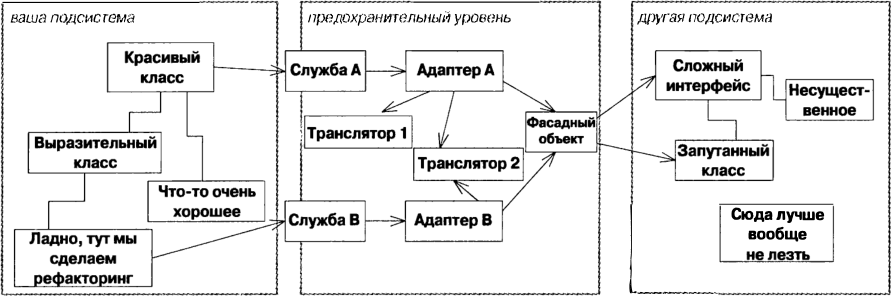
\includegraphics[width=0.9\textwidth]{anticorruptionLayer.png}
\end{center}

\subsubsection{Отдельное существование}

Паттерн <<Отдельное существование>> (Separate Ways) применяется, когда даже <<Предохранительный уровень>> неприменим (например, из-за дороговизны разработки подсистемы преобразования), или вообще в ситуациях, когда преимущества от интеграции меньше затрат на неё. <<Отдельное существование>>, как понятно из паттерна, предполагает отсутствие интеграции вообще --- вы принимаете решения игнорировать существование другого проекта и не пытаться оттуда ничего переиспользовать. 

Хороший жизненный пример применения такого паттерна --- командная работа над дипломом. В некоторых ситуациях какая-либо запланированная интеграция реализаций разных дипломов может быть очень плохой идеей, даже если несколько дипломов пишутся в одном проекте по очень похожим задачам и могут активно переиспользовать функциональность друг друга. В этом случае риски и потенциальный ущерб от их осуществления существенно превышают возможные преимущества от интеграции, даже если сама интеграция и недорога --- кто-то из участников может уйти в академ или просто не осилить, остальным тоже уходить в академ?

\subsubsection{Служба с открытым протоколом}

Паттерн <<Служба с открытым протоколом>> (Open Host Service) --- это что-то вроде <<Заказчик-Поставщик>> со стороны поставщика, у которого уж очень много заказчиков, так что приглашать их всех на planning-сессии и учесть все их пожелания не получится. В этом случае рекомендуется в каком-то смысле вообще не рассматривать <<хотелки>> заказчиков (за исключением требований) и строить модель предметной области самим. После чего предоставить публичный интерфейс, представляющий эту модель, и опубликовать саму модель вместе с интерфейсом (обычно в виде текстовой документации). А заказчикам предлагается самим подстраиваться под опубликованную модель (применяя паттерн <<Конформист>>, или <<Предохранительный уровень>>, если они сильно недовольны).

Пример использования такого подхода --- это большинство публичных REST-сервисов, таких как VK API, Google Drive API и т.д. Публикуются сами сервисы и документация, в которой объясняется, какими сущностями и как эти сервисы манипулируют. При этом обратите внимание, что модель предметной области и единый язык опубликованного сервиса может отличаться от модели предметной области и единого языка, используемого в его реализации. Как правило, <<внешнюю>> модель стараются сделать как можно более простой, тогда как в реализации можно (и часто требуется) разгуляться по полной.

\subsubsection{Общедоступный язык}

Паттерн <<Общедоступный язык>> (Published Language) применяется, когда предметная область достаточно популярна, чтобы в ней появилось очень много <<заказчиков>> и много <<поставщиков>>. Тогда рекомендуется общими усилиями разработать модель предметной области, удовлетворяющую всех поставщиков, стандартизовать её и навязать заказчикам. Эта общая модель предметной области не должна навязывать ничего касательно реализации и должна быть максимально простой, но вместе с тем достаточно выразительной. Для реализации компонентов и сервисов в рамках этой модели могут использоваться свои ограниченные контексты (и не одни), не обязательно совпадающие с опубликованной моделью. Общая модель служит скорее языком и общей средой для общения различных систем в предметной области. 

Примеры применения такого подхода --- это языки программирования (например, компиляторы C++ поставляются несколькими известными производителями, но это более-менее один язык, то же с UML) и отраслевые стандарты --- например, стандарты хранения и передачи медицинских данных, типовые архитектуры авионики или автомобильного бортового программного обеспечения. Стандарты фиксируют общую понятийную базу и терминологию (единый язык) и связь между понятиями (модель предметной области), которым должны следовать все, работающие по стандарту. 

Кстати, стандарт IEEE 1016-2009, упоминавшийся в первой лекции этого курса, --- это как раз пример стандарта с общедоступным языком. Там прямо с использованием UML описывалась предметная область архитектурных видов и предлагался единый язык.

\subsubsection{Сравнение подходов к интеграции}

Взаимосвязь различных  подходов к интеграции ограниченных контекстов описывает рисунок из книги Эванса: 

\begin{center}
    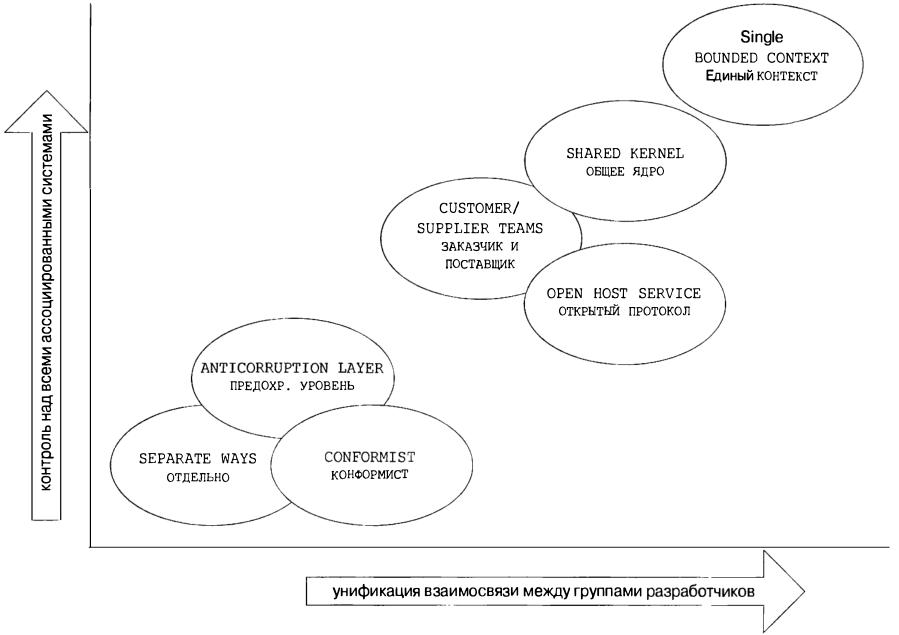
\includegraphics[width=0.8\textwidth]{integrationPatterns.png}
\end{center}

В правом верхнем углу находится полная интеграция --- когда команды работают в едином ограниченном контексте. Это требует максимальной взаимосвязи между группами разработчиков (на самом деле, по факту это должна быть одна команда) и максимального контроля над кодом (на самом деле, кодовая база должна быть полностью подвластна команде). Чуть слабее требования у паттерна <<Общее ядро>>. Дальше стоят <<Заказчик-Поставщик>> и <<Открытый протокол>> --- при этом <<Заказчик-Поставщик>> позволяет влиять на компонент, от которого мы зависим, <<Открытый протокол>> в меньшей степени, зато требует существенно больше документации (поэтому требуется больше коммуникации, хоть и односторонней).

В левом нижнем углу находятся паттерны, применяемые, кода всё плохо. <<Предохранительный уровень>> --- кода мы хотим писать какой-то код, чтобы защитить своё миропонимание от навязанного третьесторонним компонентом (так что требует много кода), <<Конформист>> --- когда не хотим, но тогда нам надо болше разбираться в миропонимании компонента (оттого больше коммуникации, даже если она заключается в чтении документации и кода). И наконец, <<Отдельное существование>> не требует ни коммуникации, ни какого-либо контроля, но и интеграции никакой не даёт.

\subsection{Пример: унификация слона}

Небольшой метафорический, но на самом деле очень жизненный пример применения паттернов интеграции из книги Эванса основывается на стихотворении <<Слепцы и слон>> Дж. г. Сакса (1816--1887):

\begin{verse}
    Шесть седовласых мудрецов \\
    Сошлись из разных стран. \\
    К несчастью, каждый был незряч, \\
    Зато умом блистал. \\
    Они исследовать слона \\
    Явились в Индостан. \\!

    Один погладил бок слона. \\
    Довольный тем сполна, \\
    Сказал он: ``Истина теперь \\
    Как божий день видна: \\
    Предмет, что мы зовем слоном, ­\\
    Отвесная стена!'' \\!

    А третий хобот в руки взял \\
    И закричал: ``Друзья! \\
    Гораздо проще наш вопрос, \\
    Уверен в этом я! \\
    Сей слон --- живое существо, \\
    А именно змея!'' \\!

    Мудрец четвертый обхватил \\
    Одну из ног слона \\
    И важно молвил: ``Это ствол, \\
    Картина мне ясна! \\
    Слон --- дерево, что зацветет, \\
    Когда придет весна!'' \\!

    Тем временем шестой из них \\
    Добрался до хвоста. \\
    И рассмеялся от того, \\
    Как истина проста. \\
    ``Ваш слон --- веревка. Если ж нет \\
    Зашейте мне уста!'' \\!

    А как известно, мудрецам \\
    Присущ упрямый нрав. \\
    Спор развязав, они дошли \\
    Едва ль не до расправ. \\
    Но правды ни один не знал, \\
    Хотя был в чем-то прав.
\end{verse}

Шесть мудрецов --- это шесть команд разработчиков, работающих над одним проектом в шести ограниченных контекстах. Посмотрим, как они могли бы постепенно интегрировать свои контексты, улучшая в процессе интеграции качество модели и своё понимание предметной области.

Первый вариант интеграции --- отсутствие интеграции как таковой, почти как в оригинальном стихотворении. Это соответствует паттерну <<Раздельное существование>>, когда каждый мудрец имеет свою точку зрения, придерживается её и не лезет в другие ограниченные контексты. Системы не могут интегрироваться друг с другом и их модели предметной области радикально различны:

\begin{center}
    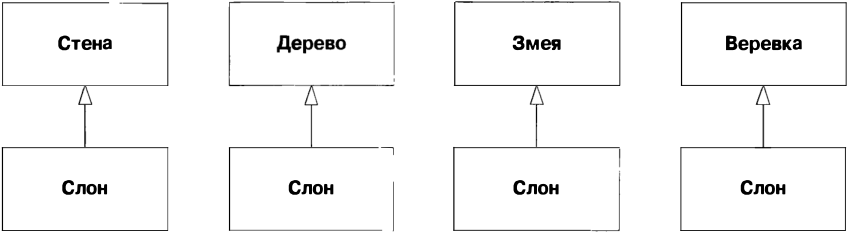
\includegraphics[width=0.8\textwidth]{elephantSeparateWays.png}
\end{center}

Некоторая минимальная интеграция могла бы быть получена с помощью паттерна <<Предохранительный уровень>>. Каждый мудрец всё ещё считает, что остальные понимают предметную область неправильно, но они могут договориться о схеме трансляции между понятиями: 

\begin{center}
    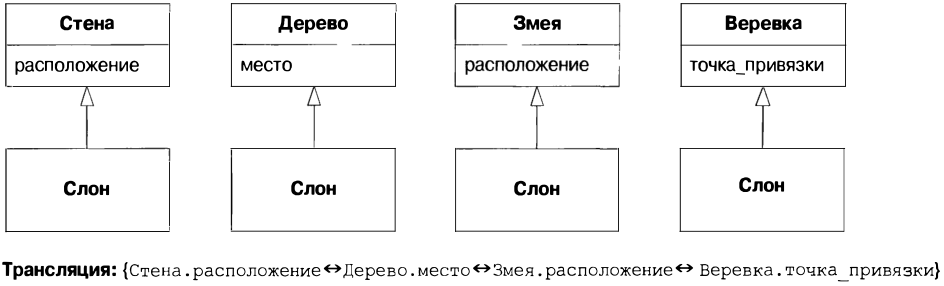
\includegraphics[width=0.9\textwidth]{elephantAnticorruptionLayer.png}
\end{center}

Теперь у всех моделей есть некоторые свойства, которые по оговоренным заранее правилам могут преобразовываться друг в друга. Не всегда это преобразование тривиально, не всегда сохраняет все данные, не всегда имеет смысл в рамках <<настоящей>> предметной области, но всё-таки позволяет системам работать совместно. Например, мудрец, считающий слона стеной, может определить расположение стены, которое может быть так или иначе транслировано в точку привязки верёвки для мудреца, который считает слона верёвкой. 

Стоит отметить, что и в реальной жизни <<настоящая>> предметная область далеко не очевидна, особенно в начале разработки, особенно если разработка ведётся в сфере, далёкой от жизненного опыта разработчиков (например, информационная система для автомобильного завода или даже информационная система поддержки учебных практик СПбГУ). Если несколько команд работают над одной областью и анализируют её независимо (например потому, что относятся к разным организациям и просто не знают о существовании друг друга), они будут действовать в точности как слепые мудрецы и проблемы на первых этапах интеграции, если она начнётся, практически неизбежны.

Следующий этап --- это выделение общего ядра. В оригинальном стихотворении мудрецы просто разругались, в мире программирования всё же более типична ситуация, когда команды продолжают работать вместе и находят общие фрагменты своих моделей, что становится основой интеграции:

\begin{center}
    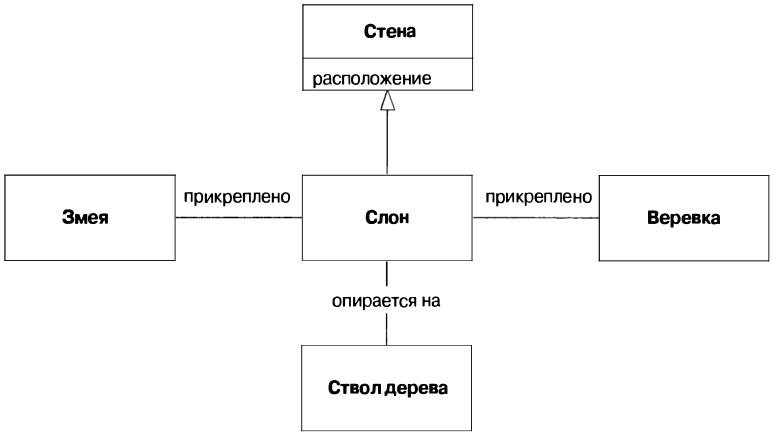
\includegraphics[width=0.8\textwidth]{elephantSharedKernel.png}
\end{center}

Тут мудрецы уже поняли, что говорят по сути об одном, но каждый всё ещё наделяет слона своими своствами, специфичными для его точки зрения. Тем не менее, они уже могут рассуждать в терминах общей и понимаемой ими однозначно сущности <<Слон>>. При этом одному из мудрецов повезло и его класс <<Стена>> был принят как предок для класса <<Слон>>, так что мудрецы согласились, что у слона есть расположение. Но это не значит, что класс <<Стена>> сам принадлежит смысловому ядру: всё, что от него можно унаследовать, то есть состояние, поведение и инварианты --- да, безусловно, но вряд ли мудрецы бы согласились включить в единый язык общего ядра тот факт, что слон является стеной. А в DDD общий язык важнее технических соображений.

Ну и последний этап интеграции --- когда мудрецы достигают полного согласия и формируют единый ограниченный контекст:

\begin{center}
    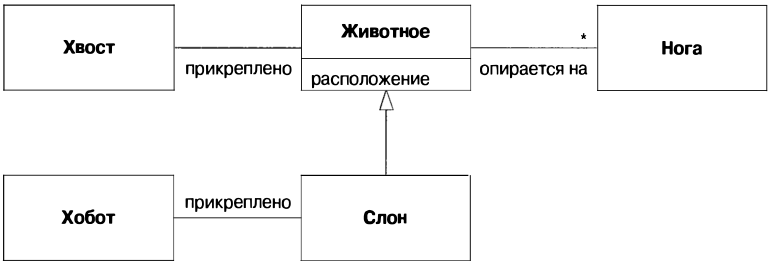
\includegraphics[width=0.8\textwidth]{elephantSingleBoundedContext.png}
\end{center}

Таким образом, команды разработчиков, в отличие от мудрецов, с помощью постепенной интеграции всё-таки смогли установить истину и собрать из фрагментов единую модель предметной области, в которой могут работать, пока снова не разругаются.

\section{Смысловое ядро}

Ключевой момент предметно-ориентированного проектирования больших систем --- это выделение их самой содержательной части, вынесение из неё всего, непосредственно к ней не относящегося, и акуратный её дизайн. Эта содержательная часть предметной области называется \textit{смысловое ядро} (Core Domain) --- это то, что, собственно, делает систему ценной. То, за что, собственно, заказчики платят деньги. Например, в любой информационной системе есть библиотека для работы с базой данных, скорее всего, какая-то сетевая часть, скорее всего, какой-то UI. Но полезна информационная система только тогда, когда правильно моделирует данные и бизнес-процессы заказчика. Или компьютерная игра --- вы можете потратить кучу времени на реализацию сохранения-загрузки, но купят игру либо из-за интересной игровой механики, либо из-за хорошего дизайна, либо ещё из-за чего-то, с сохранением и загрузкой не связанного. Сохранение и загрузка тоже важны, и без них игру не купят, но это не главное.

Только смысловое ядро фактически составляет know-how, то, что выделяет ваш продукт на фоне конкурентов и то, что представляет настоящую ценность, всё остальное в принципе можно смело выложить в open source (а лучше взять из open source, потому что наверняка уже десять раз реализовано). Пожтому смысловое ядро должно быть самой проработанной частью системы. Причём, ирония состоит в том, что опытные программисты не любят заниматься смысловым ядром, потому что оно требует глубокого погружения в предметную область. Гораздо приятнее заниматься базами данных или UI и написать потом в резюме длинный список технологий, которыми ты мастерски владеешь, чем написать в резюме, что ты прекрасно разбираешься в работе логистических компаний (и тогда тебя трудоустроят те две-три компании в мире, которые делают свой бизнес на автоматизации в сфере логистики) или ты эксперт в размножении тушканчиков и умеешь строить отличные предметно-ориентированные модели.

С таким мировоззрением надо бороться. На самом деле, работать на резюме в плане изучения стеков технологий может быть полезно, пока вы junior developer, но ближе к позиции senior уже стратегически невыгодно. Богатый технический бэкграунд к этому моменту постепенно обесценится из-за естественной смены модных технологий, и с вами на рынке труда будут конкурировать junior-ы, которые на новых технологиях выросли, и поэтому знают их лучше вашего. Да и вряд ли вы к тому времени будете хотеть juniorскую зарплату. А вот специализация в некоторой предметной области junior-ам недоступна, поскольку требует массы времени и усилий уже после базового образования, и, хоть и сужает возможности трудоустройства, делает вас ценным специалистом, которого самого приглашают на работу, причём на очень высокую зарплату (потому что такие специалисты редки). В мире миллионы Java-программистов, но программист, шарящий в размножении тушканчиков, возможно, один, и если кому-то он понадобится, за него отдадут любые деньги. Например, молодых выпускников матмеха, успевших специализироваться в компьютерной криминалистике, несмотря на небольшое количество работодателей в этой сфере, перекупали друг у друга у меня на глазах.

Смысловое ядро, поскольку оно самая важная часть системы, должно быть как можно меньше (чтобы с ним легче было работать) и чётко отделённым от остальных компонентов системы. Процесс выделения смыслового ядра Эванс называет \textit{дистилляцией} и приводит несколько дельных советов про то, как это делать.

Первый приём, позволяющий выделить смысловое ядро --- это Domain Vision Statement. Domain Vision Statement --- это короткий документ (примерно на одну страницу), описывающий смысловое ядро и его полезность. Обычно его имеет смысл делать в самом начале проекта, вместе с описанием проекта вообще. В реальной жизни ни разу такого не видел, однако видел ``устав проекта'', где, в частности, и описывается то, что должно быть в Domain Vision Statement. Тем не менее, охотно поверю в полезность такого документа. Смысл тут в том, чтобы документ был коротким и ёмким, не надо описывать архитектуру ядра, надо описать, что оно умеет и зачем оно.

Выделенное ядро (Highlighted Core) --- это способ уже на готовой модели обозначить смысловое ядро. Бывает двух видов. Первый --- \textit{дистилляционный документ} --- это 3-7 страниц текста про то, что составляет смысловое ядро и как его элементы взаимодействуют друг с другом. По сути, развёрнутый Domain Vision Statement, с архитектурой смыслового ядра, как правило, часть архитектурной документации. Второй --- Flagged Core --- это когда элементы ядра выделены на существующей модели, например, специальным стереотипом или даже просто цветом. 

\end{document}